\documentclass[12pt,preprint]{aastex}

\usepackage{verbatim}
\usepackage{color}
\usepackage[normalem]{ulem} % for striking out with \sout
% A comment block

%\newcommand{\comment}[1]{}

% For color
\newcommand{\mpname}[1]{#1_color.eps}
\newcommand{\clraitoff}{red}
\newcommand{\lumblack}{(black)}
\newcommand{\lumblue}{(blue)}
\newcommand{\lumred}{(red)}
\newcommand{\vdisred}{(red-dashed curve)}
\newcommand{\vdisblue}{(blue-solid curve)}

% For bw
%\newcommand{\mpname}[1]{#1.eps}
%\newcommand{\clraitoff}{}
%\newcommand{\lumblack}{}
%\newcommand{\lumblue}{}
%\newcommand{\lumred}{}
%\newcommand{\vdisred}{(dashed curve)}
%\newcommand{\vdisblue}{(solid curve)}

\newcommand{\umag}{$u$}
\newcommand{\gmag}{$g$}
\newcommand{\rmag}{$r$}
\newcommand{\imag}{$i$}
\newcommand{\zmag}{$z$}
\newcommand{\gmr}{$g-r$}



\newcommand{\gammat}{$\gamma_T$}
\newcommand{\gammacross}{$\gamma_\times$}
\newcommand{\deltasig}{$\Delta \Sigma$}
\newcommand{\deltaplus}{$\Delta \Sigma_+$}
\newcommand{\deltacross}{$\Delta \Sigma_\times$}
\newcommand{\deltarho}{$\Delta \rho$}
\newcommand{\movr}{$M(<r)$}
\newcommand{\sigmacrit}{$\Sigma_{crit}$}

\newcommand{\photoz}{photo-z}
\newcommand{\photozs}{photo-zs}

\newcommand{\tlum}{$L^{tot}$}
\newcommand{\tngal}{$N_{gal}^{tot}$}

\newcommand{\lstarlim}{$0.4 L_*$}
\newcommand{\lvir}{$L_{200}$}
\newcommand{\lvirtot}{$L^{tot}_{200}$}
\newcommand{\mvir}{$M_{200}$}
\newcommand{\nvir}{$N_{200}$}
\newcommand{\rvirgal}{$r_{200}^{gals}$}
\newcommand{\rvirmass}{$r_{200}^{mass}$}

\newcommand{\deltamtol}{$\Delta M/\Delta L$}
\newcommand{\deltam}{$\Delta M$}
\newcommand{\deltal}{$\Delta L$}

\newcommand{\deltamvir}{$\Delta M_{200}$}
\newcommand{\deltalvir}{$\Delta L_{200}$}

\newcommand{\mtolmax}{$(\Delta M/\Delta L)_{22\mathrm{Mpc}}$}
\newcommand{\mtolasym}{$(\Delta M/\Delta L)_{asym}$}
\newcommand{\mtolvir}{$(\Delta M/\Delta L)_{200}$}
\newcommand{\bmtol}{$b^2_{M/L}$}
\newcommand{\bmtolinv}{$b^{-2}_{M/L}$}

\newcommand{\ngal}{$N_{gal}$}
\newcommand{\maxbcg}{MaxBCG}
\newcommand{\numNgalBins}{12}
\newcommand{\numLumBins}{16}

\newcommand{\tngalAperture}{2$h^{-1}$ Mpc}

\newcommand{\photo}{\texttt{PHOTO}}
\newcommand{\astrop}{\texttt{ASTRO}}
\newcommand{\mt}{\texttt{MT}}
\newcommand{\spectro}{\texttt{SPECTRO}}
\newcommand{\spectroone}{\texttt{SPECTRO1d}}
\newcommand{\spectrotwo}{\texttt{SPECTRO2d}}
\newcommand{\target}{\texttt{TARGET}}

\newcommand{\lenszmax}{0.3}
\newcommand{\lenszmin}{0.05}
\newcommand{\zmean}{0.25}

\newcommand{\photoversion}{\texttt{v5\_4}}

%\def\eone{e$_1$}
%\def\etwo{e$_2$}
\newcommand{\etan}{e$_+$}
\newcommand{\erad}{e$_\times$}
\newcommand{\eclass}{\texttt{ECLASS}}
\newcommand{\eclasscut}{-0.06}
\newcommand{\gmrcut}{0.7}

\newcommand{\hrs}{$^{\mathrm h}$}
\newcommand{\minutes}{$^{\mathrm m}$}

\newcommand{\ugriz}{$u, g, r, i, z$}
\newcommand{\polarization}{polarization}

\newcommand{\wgm}{$w_{gm}$}
\newcommand{\wgg}{$w_{gg}^p$}
\newcommand{\wmm}{$w_{mm}$}
\newcommand{\xigg}{$\xi_{gg}$}
\newcommand{\ximm}{$\xi_{mm}$}
\newcommand{\xigm}{$\xi_{gm}$}

\newcommand{\numspec}{127,001}
\newcommand{\numspecvlim}{10,277}
\newcommand{\numrand}{1,270,010}
\newcommand{\numspectot}{278,192}
\newcommand{\numvdis}{49,024}
%\newcommand{\numsource}{10,259,949}
% hirata: 
\newcommand{\nummask}{1,815,043}
\newcommand{\numTenMpc}{132,473}
\newcommand{\numThirtyMpc}{101,221}
\newcommand{\numsource}{27,912,891}

\newcommand{\numpairsTenMpc}{2,670,898,177}
\newcommand{\altnumpairsTenMpc}{2.7 billion}
\newcommand{\numpairsThirtyMpc}{14,818,082,122}
\newcommand{\altnumpairsThirtyMpc}{14.8 billion}



\newcommand{\xirmax}{$\xi_{gm}(R_{max})$}


\def\eps@scaling{1.0}% 

\newcommand{\Tsn}{$(S/N)_T$}
\newcommand{\fsn}{$(S/N)_{flux}$}

\slugcomment{Last revision \today}
\shortauthors{Sheldon}
\shorttitle{Bayesian Shear Estimation}

\begin{document}

\title{On Bayesian Shear Estimation}

\author{
Erin S. Sheldon\altaffilmark{1}
}
\altaffiltext{1}{Brookhaven National Laboratory, Bldg 510, Upton, New York 11973}



\begin{abstract}

blah

\end{abstract}

\section{Introduction} \label{sec:intro}

intro

\section{Algorithm} \label{sec:algo}

algo

\section{Simulation} \label{sec:sim}

sim

\section{Results} \label{sec:results}

\begin{figure}[t] \centering
 \centering 
 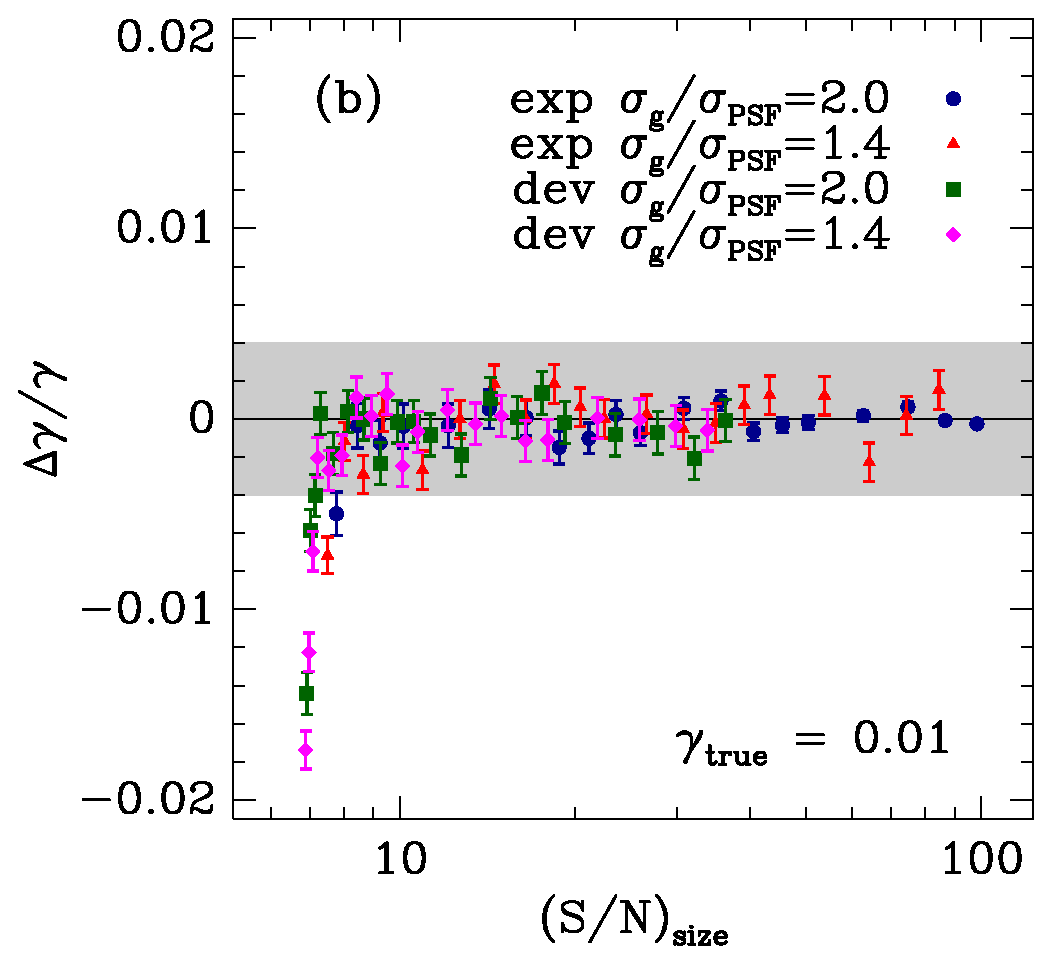
\includegraphics[scale=0.4]{figures/cbafit-geg-T-s2n.eps}
 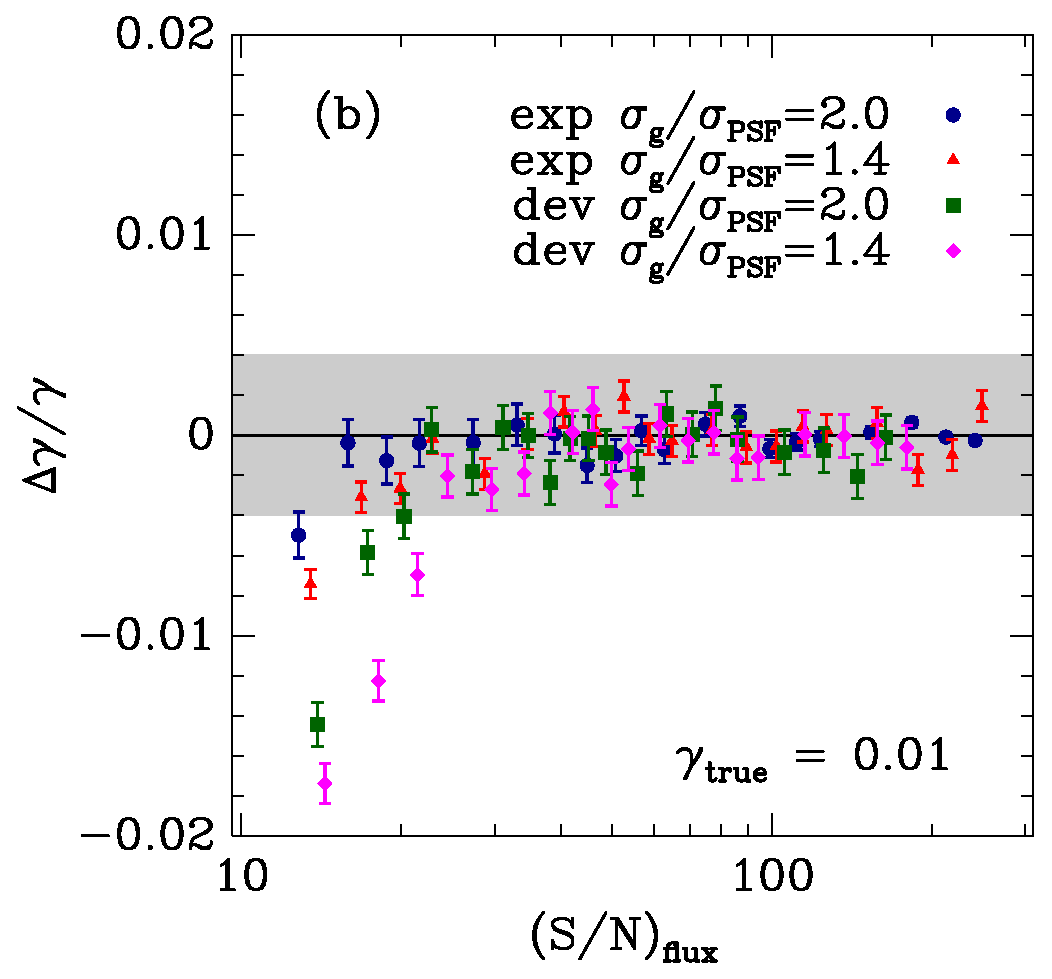
\includegraphics[scale=0.4]{figures/cbafit-geg-flux-s2n.eps}

 \caption{ Fractional error in the recovered shear for the estimator presented
     in \cite{ba13}.  The error is plotted as a function of galaxy
     signal-to-noise ratio (S/N), for various galaxy properties and two
     different measures of S/N.  In the left panel is plotted \Tsn, where the
     measure of size is $T=I_{xx} + I_{yy}$.  In the right panel is plotted
     \fsn, the signal-to-noise ratio of the total flux in the galaxy.  The flux
     and $T$ are parameters in the model fits, and the associated (S/N) is the
     ratio of measured value to error in the fit parameter.  In each panel the
     fractional error is plotted for galaxies of different size and type, as
     described in the text.  As shown in the left panel, the error depends
     uniquely on \Tsn\ for different galaxy types and sizes.  However, \fsn\ is
     not a unique descriminator for different galaxy types and sizes.   The
     \Tsn\ can be used to remove galaxies from the sample that will yield poor
 shear estimates, independent of galaxy properties, but not so \fsn.  For \Tsn$
 > 10$ this shear estimator meets the requirements for DES, shown as the grey
 band.  \label{fig:fracerr}}

\end{figure}


\begin{figure}[t] \centering
 \centering 
 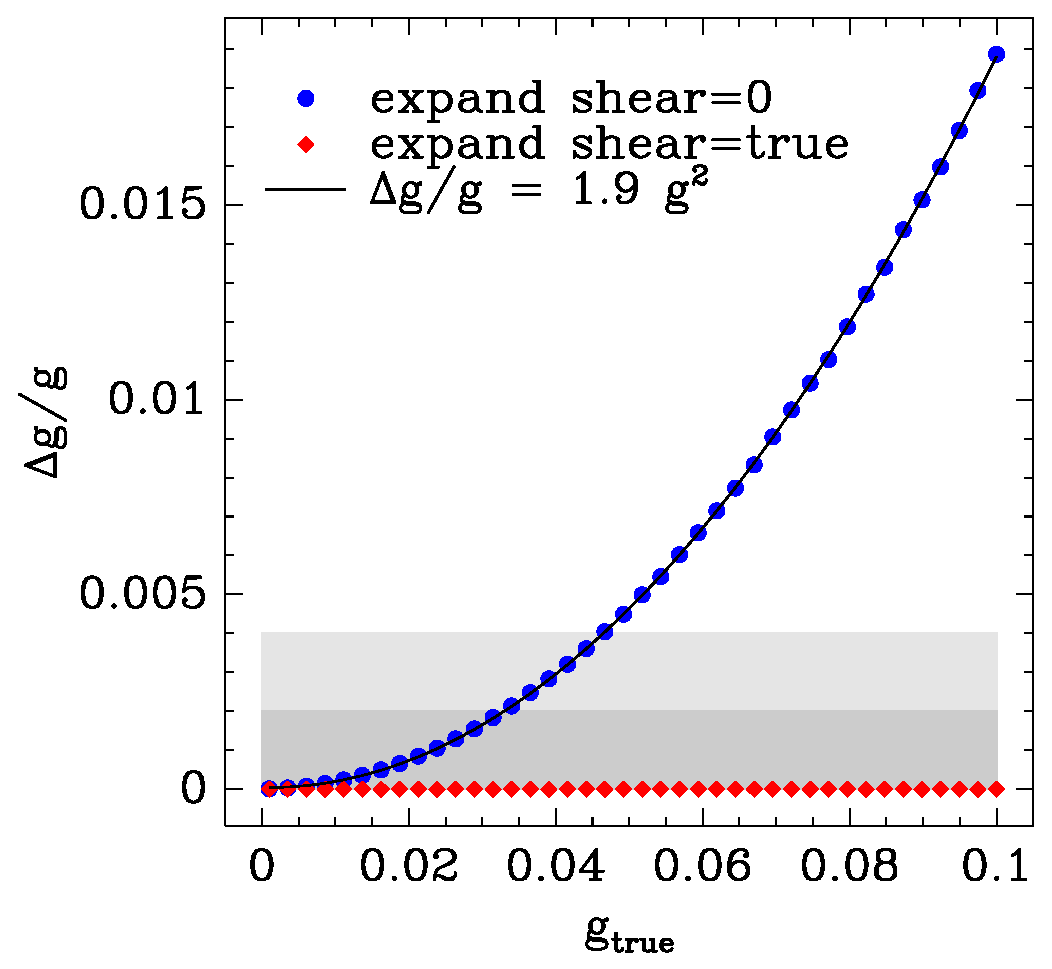
\includegraphics[scale=0.6]{figures/fracerr-vs-shear.eps}

 \caption{Fractional error in the recovered shear as a function
 of true shear, in a zero noise simulation.\label{fig:nonoise}}

\end{figure}


res

\section{Summary} \label{sec:summary}

summary

\section*{Acknowledgments}

ES is supported by DOE grant DE-AC02-98CH10886.

Thanks to Gary Bernstein, Bob Armstrong, and Anze Slosar for many useful
discussions.

\bibliographystyle{apj}
% Bib database
\bibliography{apj-jour,astroref}

\end{document}

